\documentclass[a4paper, 12pt, oneside]{article}
\usepackage[UTF8]{ctex}
\usepackage{indentfirst}
\usepackage{setspace}
\linespread{1.5}
\usepackage{mathtools}
\usepackage{hyperref}
\hypersetup{
 pdfauthor={张亚栋 10154508169},
 pdftitle={活动设计期末作业},
 pdfkeywords={幼儿园 活动设计 数理逻辑 遗传},
 pdfsubject={儿童心理},
 pdfcreator={Overleaf: https://v2.overleaf.com/}, 
 pdflang={Zh-Hans},
 colorlinks=true,
 urlcolor=cyan,
 % linkcolor=cyan
 }
\usepackage{graphicx}
\usepackage{pgffor}
\usepackage{subfigure}
\usepackage{float}
\usepackage{tikz,lipsum,lmodern}
\usepackage[most]{tcolorbox}
\usepackage{enumerate}


\title{活动设计期末作业}
\author{张亚栋 10154508169}
% \date{\today} % 2018.7.3
\date{\zhdate{2018/7/3}} 
% 感谢“LaTeX技术交流5000人群”(91940767)网友 “上海-ddswhu”QQ:1021489948 的支持

\begin{document}

\maketitle
% \thispagestyle{empty}
% \newpage

% \setcounter{page}{1}
\begin{tcolorbox}[colback=red!5!white,colframe=red!75!black]
    \begin{itemize}
        \item 主题:动物的花花衣
        \item 年龄阶段:
        \begin{enumerate}
            \item 小班(区角活动)
            \item 大班(集体教学活动)
        \end{enumerate}
        \item 初衷:\\
        各种生活现象被抽象出来形成了小学、中学及其大学的课程内容,那么在幼儿园可以反过来用这些知识来解释生活现象,学校学理论,幼儿园讲应用,学习一些基本理论是如何体现在周围环境中的。
    \end{itemize}
\end{tcolorbox}
    
\section{区角活动}
    \subsection{区角材料}
    \begin{figure}[H]
        \centering
            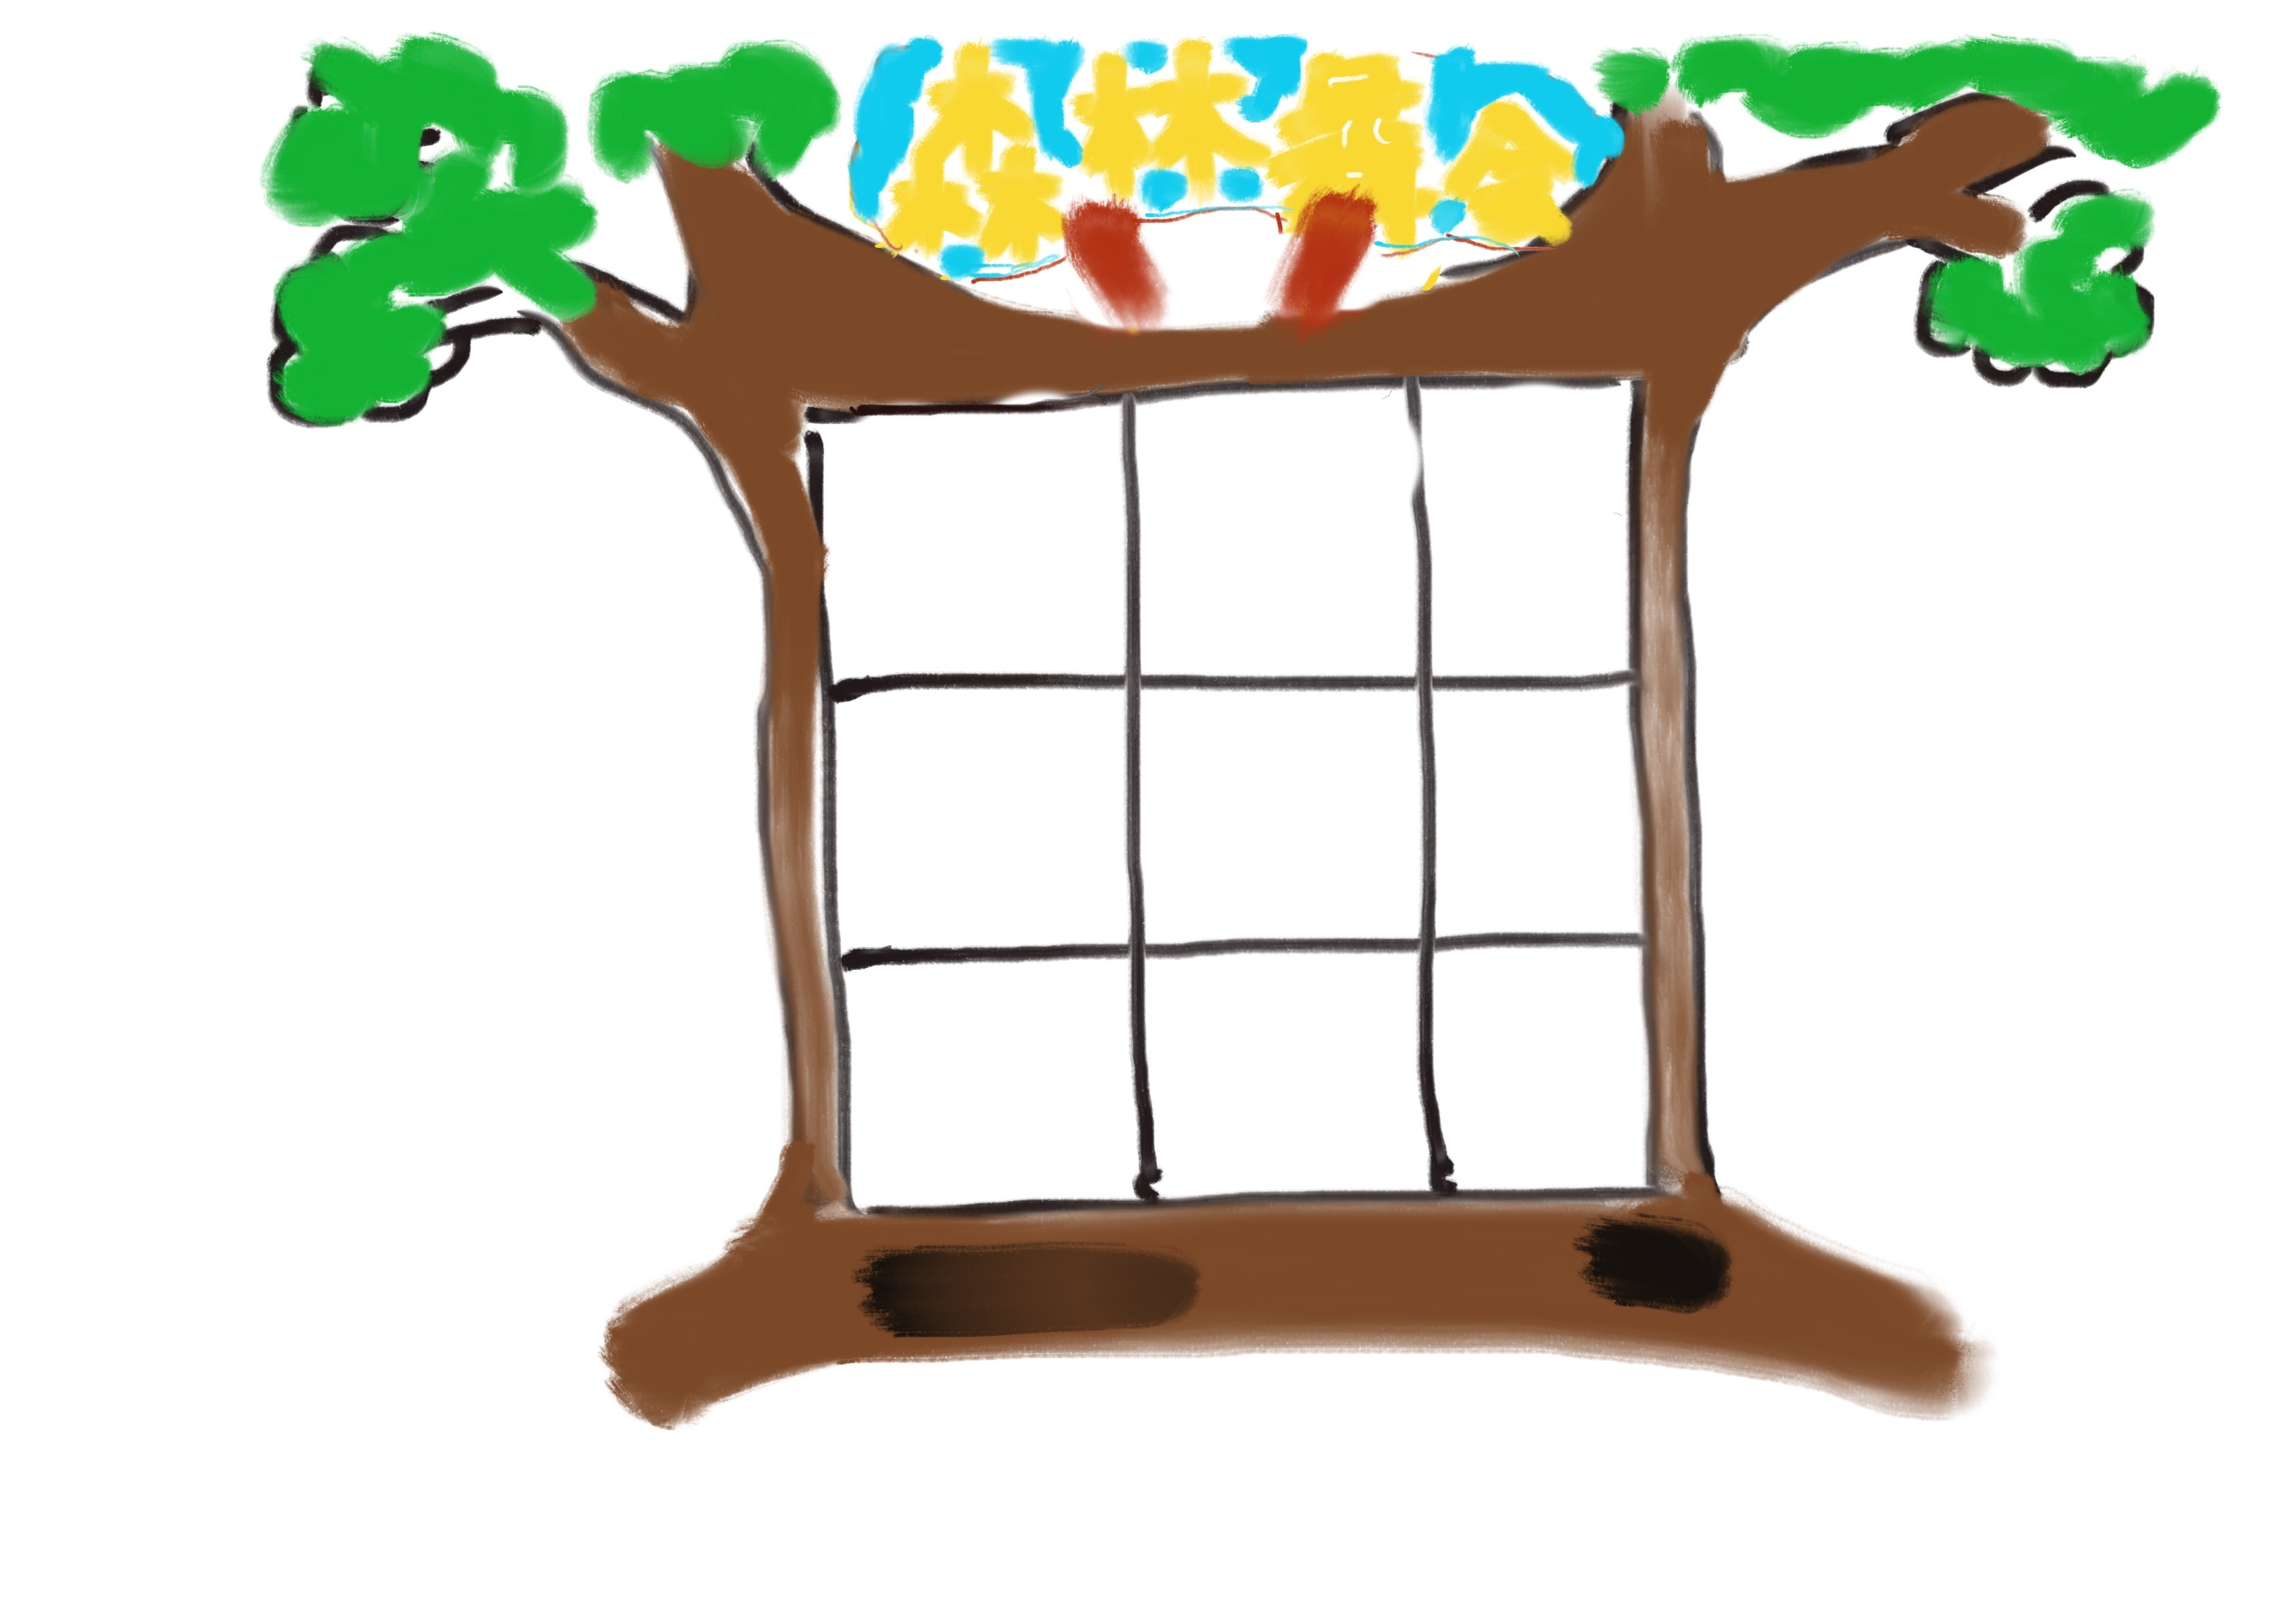
\includegraphics[width=0.5\textwidth]{images/0.jpg}
        \caption{背景}
    \end{figure}
    
    \begin{figure}[H]
        \centering
            \foreach \t in {1,2,3}
            {
                \includegraphics[width=0.2\textwidth]{images/00\t.png}~~~~~~~~
            } 
        \caption{卡片}
    \end{figure}
    
    \begin{tcolorbox}[colback=yellow!10!white,colframe=red!75!black,title=玩法介绍]
        每个格子只能填入一个动物卡片,每行每列不能相同。
    \end{tcolorbox}
    \begin{tcolorbox}[colback=yellow!10!white,colframe=red!75!black,title=设计理由]
        锻炼儿童逻辑推理能力。
    \end{tcolorbox}
    \subsection{数学原理}
        \begin{tcolorbox}[colback=red!5!white,colframe=red!75!black]
            \begin{enumerate}
                \item 为保证第 i行包含第n个动物,必须满足
                    $$
                    \begin{matrix}
                        \bigvee_{j=1}^3 ~p\left(i, j, n\right)
                    \end{matrix}
                    $$
                \item 为保证第i行包含所有动物,必须满足
                    $$
                    \begin{matrix}
                        \bigwedge_{n=1}^3\bigvee_{j=1}^3 ~p\left(i, j, n\right)
                    \end{matrix}
                    $$
                \item 为保证每一行都包含所有动物, 必须满足
                    $$
                    \begin{matrix}
                        \bigwedge_{i=1}^3\bigwedge_{n=1}^3\bigvee_{j=1}^3 ~p\left(i, j ,n\right)
                    \end{matrix}
                    $$
            \end{enumerate}
            \tcblower
            \hfill$\ast$\textbf{标注:}i表示行数,j表示列数,n表示动物数量。
        \end{tcolorbox}
        
        综上,共有$3\times3\times3=27$种不同情况。\par
        以上原理最早出现在《形式逻辑》中的集合与元素关系,并在~\href{https://www.amazon.com/Discrete-Mathematics-Its-Applications-Seventh/dp/0073383090}{\textit{Discrete Mathematics and Its Applications 7e}}~中给出具体证明及应用(数独)。
    \subsection{活动观察}
    这个活动我并没有在幼儿园去做,当时没有设计出来,在幼儿园待了那么长时间,我觉得可能我不大适合幼师岗位,学了三年还是不懂儿童,老师,对不起,我还是另谋出路!
\section{集体教学活动}
    \begin{tcolorbox}[colback=yellow!10!white,colframe=cyan!75!black,title=活动名称:]
        0
    \end{tcolorbox}
    \begin{tcolorbox}[colback=yellow!10!white,colframe=cyan!75!black,title=活动目标:]
        \begin{enumerate}
            \item 用数学模式解释农场中兔子毛色规律;
            \item 亲近小动物,了解小兔子的习性。
        \end{enumerate}
    \end{tcolorbox}
    \begin{tcolorbox}[colback=yellow!10!white,colframe=cyan!75!black,title=活动准备:]
        \begin{enumerate}
            \item 经验准备:农场参观兔子妈妈和兔宝宝
            \item 材料准备:
            \begin{enumerate}[1)]
                \item 不同毛色兔子卡片若干张
                \item 幻灯片
            \end{enumerate}
        \end{enumerate}
    \end{tcolorbox}
    \begin{tcolorbox}[colback=yellow!10!white,colframe=cyan!75!black,title=活动过程:]
        \begin{enumerate}
            \item 导入:\\
            打开幻灯片,让幼儿回忆在农场中做了哪些事?
            (参观了兔子养殖场,了解了兔子妈妈怎样生小兔子,以及不同阶段兔子宝宝生理上的变化)
            \item 看一看:\\
            给每个小朋友都分给3张卡片,让他们自己说说拿到的卡片上兔子的毛色特点。两个小朋友可以相互交换。
            \item 拼一拼:
            \begin{enumerate}[1)]
                \item 根据上次看到的兔子毛色规律,找到指定毛色的两只兔子可以生出什么毛色的宝宝。
                \item 相邻小朋友互换卡片,一方指定兔子妈妈和爸爸,让对方来找出剩余4张中哪些可以是兔子宝宝。
                \item 请两位小朋友来给大家展示他们的玩法。
            \end{enumerate}
        \end{enumerate}
    \end{tcolorbox}
    \begin{tcolorbox}[colback=yellow!10!white,colframe=cyan!75!black,title=活动延伸:]
        让小朋友们回家种豌豆,数量越多越好,看看豌豆的花色规律是怎样的。
    \end{tcolorbox}
\end{document}
